\chapter{IDE Untuk Go}

IDE (\textit{Integrated Development Environment}) merupakan peranti lunak yang 

\section{Menggunakan Vim}

Untuk menggunakan Vim, ada plugin utama serta berbagai plugin pendukung yang bisa digunakan. Sebaiknya, menggunakan \textbf{pathogen} untuk mempermudah pengelolaan berbagai plugin tersebut. Bagian ini akan menjelaskan berbagai konfigurasi serta instalasi yang diperlukan sehingga Vim bisa menjadi peranti untuk pengembangan aplikasi menggunakan Go.

\subsection{Instalasi dan Konfigurasi Pathogen}

Pathogen adalah plugin dari Tim Pope yang digunakan untuk mempermudah pengelolaan plugin. Kode sumber dari Pathogen bisa diperoleh di \url{https://github.com/tpope/vim-pathogen}. Untuk instalasi, ikuti langkah berikut:

\begin{mdframed}[style=catatan]
\begin{verbatim}
$ cd
$ mkdir .vim/autoload
$ mkdir .vim/bundle
$ cd .vim/autoload
$ wget https://raw.github.com/tpope/vim-pathogen/master/autoload/pathogen.vim
-2013-04-17 22:39:09--  https://raw.github.com/tpope/vim-pathogen/master/autoload/pathogen.vim
Resolving raw.github.com (raw.github.com)... 199.27.75.133
Connecting to raw.github.com (raw.github.com)|199.27.75.133|:443... connected.
HTTP request sent, awaiting response... 200 OK
Length: 11730 (11K) [text/plain]
Saving to: ‘pathogen.vim’

100%[=========================================================================
===================================================>] 11,730      50.3KB/s   in 0.2s   

2013-04-17 22:39:11 (50.3 KB/s) - ‘pathogen.vim’ saved [11730/11730]
$ ls -la
total 20
drwxr-xr-x 2 bpdp bpdp  4096 Apr 17 22:39 .
drwxr-xr-x 5 bpdp bpdp  4096 Apr 17 22:21 ..
-rw-r--r-- 1 bpdp bpdp 11730 Apr 17 22:39 pathogen.vim
$ 
\end{verbatim}
\end{mdframed}

Setelah itu, untuk menggunakan Pathogen, letakkan aktivasinya di \$HOME/.vimrc atau di \$HOME/.vim/vimrc (saya piliah lokasi yang kedua) sebagai berikut:

\begin{mdframed}[style=catatan]
  \begin{verbatim}
  execute pathogen#infect()
  \end{verbatim}
\end{mdframed}

Setelah itu, semua plugin tinggal kita ambil dari repository (bisa dari github, bitbucket, dan lain-lain) langsung di-copy satu direktori ke direktori \$HOME/.vim/bundle.

\subsection{Instalasi dan Kofigurasi Plugin Golang dan Plugin Pendukung}

Setelah selesai melakukan instalasi Pathogen, berbagai plugin yang diperlukan bisa diambil langsung dari Internet. Berikut ini adalah daftar yang digunakan penulis:
\begin{itemize}
  \item Colorschemes: untuk tema warna dari Vim. Bisa diperoleh di \url{https://github.com/flazz/vim-colorschemes}
  \item Nerdtree: untuk menampilkan file-file dalam struktur pohon di sebelah kiri sehingga memudahkan navigasi. Bisa diperoleh di \url{https://github.com/scrooloose/nerdtree}
  \item Golang: plugin utama agar Vim mengenali kode sumber Go. Bisa diperoleh di: \url{https://github.com/jnwhiteh/vim-golang.git}
\end{itemize}

Cara instalasi:

\begin{mdframed}[style=catatan]
  \begin{verbatim}
$ cd 
$ cd .vim/bundle
$ git clone <masing-masing lokasi plugin>
\end{verbatim}
\end{mdframed}

Kode sumber lengkap dari \$HOME/.vim/vimrc yang penulis gunakan bisa dilihat pada Listing~\ref{lst:vimrc} adalah sebagai berikut:

\lstset{language=Bash, caption=\$HOME/.vim/vimrc, label={lst:vimrc}}
\lstinputlisting{src/non-go/bab-02/vimrc.txt}

Hasil dari menjalankan ``vim'' atau ``gvim'' melalui shell untuk menulis kode sumber Go bisa dilihat pada Gambar~\ref{fig:vim-go}

  \begin{figure}
    \begin{center}
      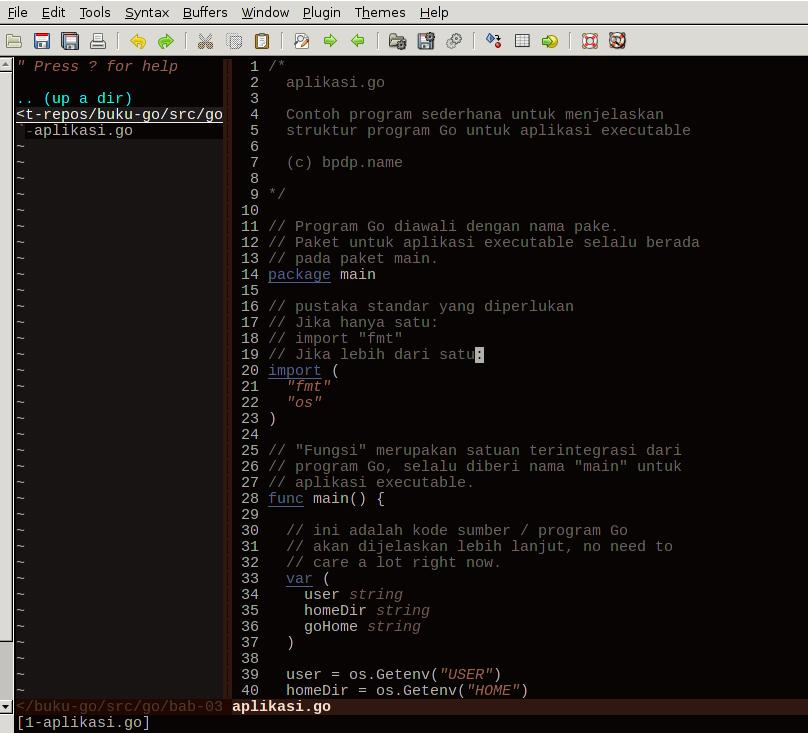
\includegraphics[scale=0.5]{images/vim-go.jpg}
    \end{center}
    \caption{Tampilan gvim untuk mengedit kode sumber Go}
    \label{fig:vim-go}
  \end{figure}

\section{Menggunakan LiteIDE}

\subsection{Download dan Instalasi}


\subsection{Membuat Proyek}


\section{Software IDE Lain}

Vim dan LiteIDE hanyalah beberapa peranti yang bisa digunakan oleh pengembang. Distribusi Go juga menyediakan dukungan untuk berbagai peranti lunak lain
